%!TEX root = ../../main.tex

Til pH måling har vi bygget vores egen sensor ved hjælp af en pH-probe.

\subsection{pH-sensor BDD}

I forhold til signaler er proben ret nem at have med at gøre da den selv producere en spænding i forhold til den væske der måles på pH værdi.

\begin{figure}[H]
	\centering
	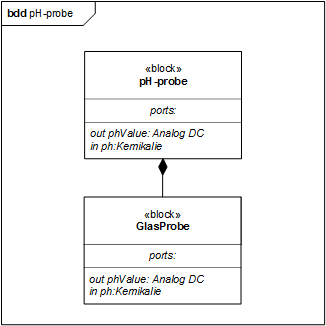
\includegraphics[width=0.7\textwidth]{Systemarkitektur/Sensor_pH/pH_Probe_BDD.png}
	\label{fig:pH-sensor BDD}
	\caption{Block Definition Diagram af pH-sensor}
\end{figure}



\subsection{pH-sensor IBD}

Igen ses simpliciteten da pH proben bare interagere med kemikalium og herefter producere en spænding.

\begin{figure}[H]
	\centering
	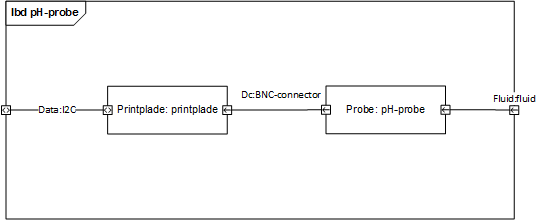
\includegraphics[width=0.7\textwidth]{Systemarkitektur/Sensor_pH/pH_Probe_IBD.png}
	\label{fig:pH-sensor IBD}
	\caption{Internal Block Diagram af pH-sensor}
\end{figure}


